\documentclass[11pt, oneside]{article}   	% use "amsart" instead of "article" for AMSLaTeX format
\usepackage{geometry}                		% See geometry.pdf to learn the layout options. There are lots.
\geometry{letterpaper}                   		% ... or a4paper or a5paper or ... 
\usepackage{graphicx}				% Use pdf, png, jpg, or eps§ with pdflatex; use eps in DVI mode
								% TeX will automatically convert eps --> pdf in pdflatex		
\usepackage{amssymb}
\usepackage{amsmath}
\usepackage{parskip}
\usepackage{color}
\usepackage{hyperref}

\graphicspath{{/Users/telliott_admin/Tex/png/}}
% \begin{center} 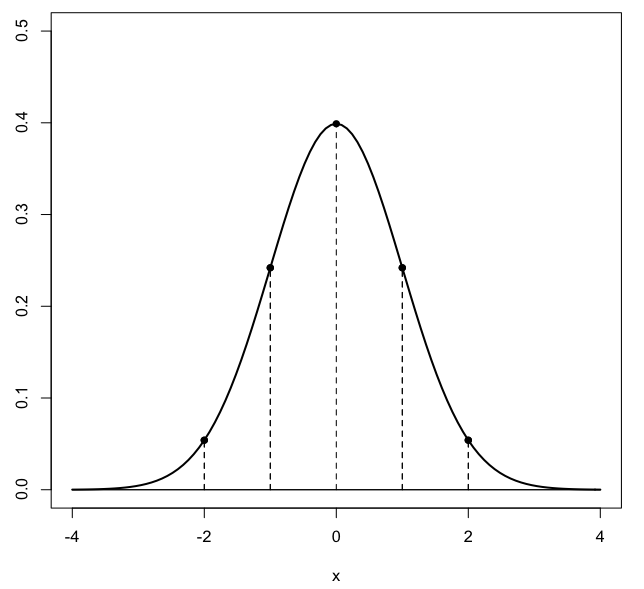
\includegraphics [scale=0.4] {gauss3.png} \end{center}

%break
\title{Line integrals}
\date{}

\begin{document}
\maketitle
\Large

\label{sec:line_integrals}

A line integral sums the values taken on by a specified function of $x$ and $y$ in $\mathbb{R}^2$, or $x,y,z$ in $\mathbb{R}^3$, evaluated at a large number positions $n$ along a particular curve, in the limit as $n \rightarrow \infty$.  

Despite the involvement of $x$ and $y$ (and perhaps $z$), a line integral is an integral of a single variable.  Because the points are all \emph{on the curve}, they can be related.  In many cases $x$ and $y$ will be parametric equations (functions of a parameter like $t$), or we might just express $y$ in terms of $x$.  In any case, the integral will be of a single variable.

A simple application of a line integral is to find the length of a curve.  A more sophisticated one yields the work done when moving along a curve, or the flux across a curve, and there are certainly others.

The basic formula can be derived by doing algebra with differentials.  Think of a small element of the curve's path, $ds$, as a right triangle with side lengths $dx$ and $dy$.  
\begin{center} 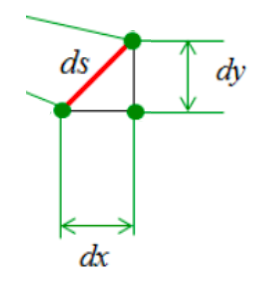
\includegraphics [scale=0.4] {path_element.png} \end{center}

Then Pythagoras tells us that

\[ ds^2 = dx^2 + dy^2 \]

We "divide and multiply" on the right by $dx^2$ to give

\[ ds^2 = [1 + \frac{dy^2}{dx^2}] \ dx^2 \]

then take the square root

\[ ds = \sqrt{1 + (\frac{dy}{dx})^2} \ dx \]
\[ ds = \sqrt{1 + (y')^2} \ dx \]

\subsection*{Example 0}
Here is one where we already know the answer:  the arc length along the boundary of the circle of radius $R$ in the first quadrant.  Again, the formula is
\[ ds = \sqrt{1 + (\frac{dy}{dx})^2} \ dx \]
So we want
\[ L = \int ds = \int_0^R  \sqrt{1 + (\frac{dy}{dx})^2} \ dx \]
The circle is
\[ x^2 + y^2 = R^2 \]

By implicit differentiation, we easily obtain
\[ 2x \ dx + 2y \ dy = 0 \]
\[ \frac{dy}{dx} = -\frac{x}{y} \]
\[ (\frac{dy}{dx})^2 = \frac{x^2}{y^2} \]
So the integral is
\[ = \int_0^R  \sqrt{1 + \frac{x^2}{y^2}} \ dx \]
\[ = \int_0^R \frac{1}{y}  \sqrt{y^2 + x^2} \ dx \]
\[ = R \int_0^R \frac{1}{y}  \ dx \]
\[ = R \int_0^R \frac{1}{\sqrt{R^2-x^2}}  \ dx \]

This can be solved by a trig substitution:
\[ x = R \sin t \]
\[ dx = R \cos t \ dt \]
\[ \sqrt{R^2 - x^2} = R \cos t \]
So we have
\[ = R \int \frac{1}{R \cos t} R \cos t \ dt = R t \]
The slightly tricky part is the limits on $t$.  The lower limit was $x=0$, so now we need $R \sin t = 0$, so $t=0$.  And the upper limit was $x=R$, so now we need $R \sin t = R$ so $t = \pi/2$.  The integral is $\pi R/2$ and the whole circumference is $4$ times that or $C = 2 \pi R$.

Another, simpler way to do this calculation is to use the parametrized circle ($x = \cos \theta, y = \sin \theta$).  Go back to the original definition of the element of arc $ds$:

\[ ds^2 = dx^2 + dy^2 \]
\[ L = \int ds = \int \sqrt{dx^2 + dy^2} \]
\[ = \int \sqrt{\cos^2 \theta + \sin^2 \theta} \ d \theta \]
\[ = \int \ d \theta \]

Here, we can just go all the way around the circle from $\theta = 0 \Rightarrow 2 \pi$.  And for a circle of radius $a$ we have $a \cos \theta$ and $a \sin \theta$ which gives a factor of $a^2$ under the square root, yielding an extra factor of $a$ in the end.

\subsection*{example 1}
Consider
\[ y = x^2 \]
\[ \frac{dy}{dx} = 2x \]
\[ ds = \sqrt{1 + (\frac{dy}{dx})^2} \ dx \]
\[ ds =  \sqrt{1 + 4x^2} \ dx \]

The arc length is the integral of $ds$

\[ L = \int  \sqrt{1 + 4x^2} \ dx \]
\[ = 2 \int  \sqrt{(\frac{1}{2})^2 + x^2} \ dx \]

This will be a minor challenge (see trig substitutions).  Rather than struggle with it, just set $a = \frac{1}{2}$ and look up the answer in a table of integrals

\[ \int  \sqrt{a^2 + x^2} \ dx  = \frac{x}{2}\sqrt{a^2 + x^2} + \frac{a^2}{2} \ln \ | \ x + \sqrt{a^2 + x^2} \ | \]

substitute back for $a = 1/2$

\[ \frac{x}{2}\sqrt{\frac{1}{4} + x^2} + \frac{1}{8} \ln \ | \ x + \sqrt{\frac{1}{4} + x^2} \ | \]

Suppose the limits are $x=1$ and $x=0$.  At the upper limit, we have

\[ \frac{1}{2}(\sqrt{1.25}) + \frac{1}{8} \ \ln \ (1 + \sqrt{1.25}) \] 
\[ \sqrt{1.25} \approx 1.118  \]
\[ \ln (2.118) \approx 0.7505 \]
\[ (0.5)(1.118) + (0.125)(0.7505) = 0.559 + 0.0938 = 0.6528 \]

while at the lower limit the first term is $0$ and the second is

\[ \frac{1}{8}\  \ln \frac{1}{2} = - (0.125)\  \ln 2 = - (0.125)(0.693) = -0.0866 \] 

Subtracting

\[ 0.6528 + 0.0866 = 0.7394 \]

Remembering the factor of two we get $1.4788$

Not exactly pretty, but it works.  Check by numerical integration

\begin{verbatim}
import scipy
f = lambda x: x**2
scipy.integrate.quad(f,0,1)
\end{verbatim}
This check gives the expected result $ 0.33333..$

\begin{verbatim}
g = lambda x: sqrt(1 + 4*x**2)
scipy.integrate.quad(g,0,1)
\end{verbatim}
results in $1.47894$

\subsection*{example 2}
Consider the ellipse
\[ y^2 + 2x^2 = 2 \]
\[ y = \sqrt{2 - 2x^2} \]
By implicit differentiation:
\[ 2y \ dy + 4x \ dx = 0 \]
\[ \frac{dy}{dx} = -\frac{2x}{y} \]
 Integrate the path element $ds$:
\[ L = \int ds \]
\[ = \int \sqrt{1 + (\frac{dy}{dx})^2} \ dx \]
\[ = \int \sqrt{1 + \frac{4x^2}{y^2}} \ dx  \]
\[ = \int \sqrt{\frac{4x^2 + y^2}{y^2}} \ dx  \]
\[ = \int \sqrt{\frac{2 + 2x^2}{2 - 2x^2}} \ dx = \int \sqrt{\frac{1 + x^2}{1 - x^2}} \ dx  \]

This can't be solved in "closed form."  The length of an ellipse can only be computed numerically.

Take one-quarter of the perimeter.  Let $x$ range from $x = 0$ ($y = \sqrt{2}$) to $x = 1$ ($y = 0$). 

\begin{verbatim}
>>> from math import sqrt
>>> def f(x):
...     r = (1 + x**2)*1.0/(1 - x**2)
...     return sqrt(r)
... 
>>> from scipy.integrate import quad
>>> quad(f,0,1)
(1.9100988945138324, 7.71731567539291e-11)
\end{verbatim}

$1.91$ is the expected result.



\end{document}